% !TEX root =../thesis-letomes.tex

\chapter{Physical Modelling}
We need a chapter to formulate our hypotheses, and generally give a before-the-fact run-down of what the project and report will be like.

\section{CM-Centric Restricted 3-Body System (Earth-Moon)}

\subsection{Equations of Motion}

\subsection{Numerical Algorithm}


\section{Heliocentric Restricted 4-Body System (Sun-Earth-Mars)}
Simulating orbit from Earth to Mars requires a new model with at least four bodies: Sun, Earth, Mars and the Spacecraft. The coordinate system will be heliocentric and in spherical coordinates, and restricted meaning that the mass of the spacecraft is considered negligible compared to compared to the celestial masses, so we call this system the ``Heliocentric Restricted N-Body'' system. We will derive the equations of motion of the spacecraft by using Hamilton's equations, which naturally gives us a set of coupled first-order differential equations, and a set of conserved quantities as ``generalized momenta''.

\subsection{Spherical Coordinate System}
We adopt the spherical coordinate system which customary in astrodynamics. The conventions used is in \cref{fig:3D_Spherical}.

\begin{figure}[ht]
    \centering
    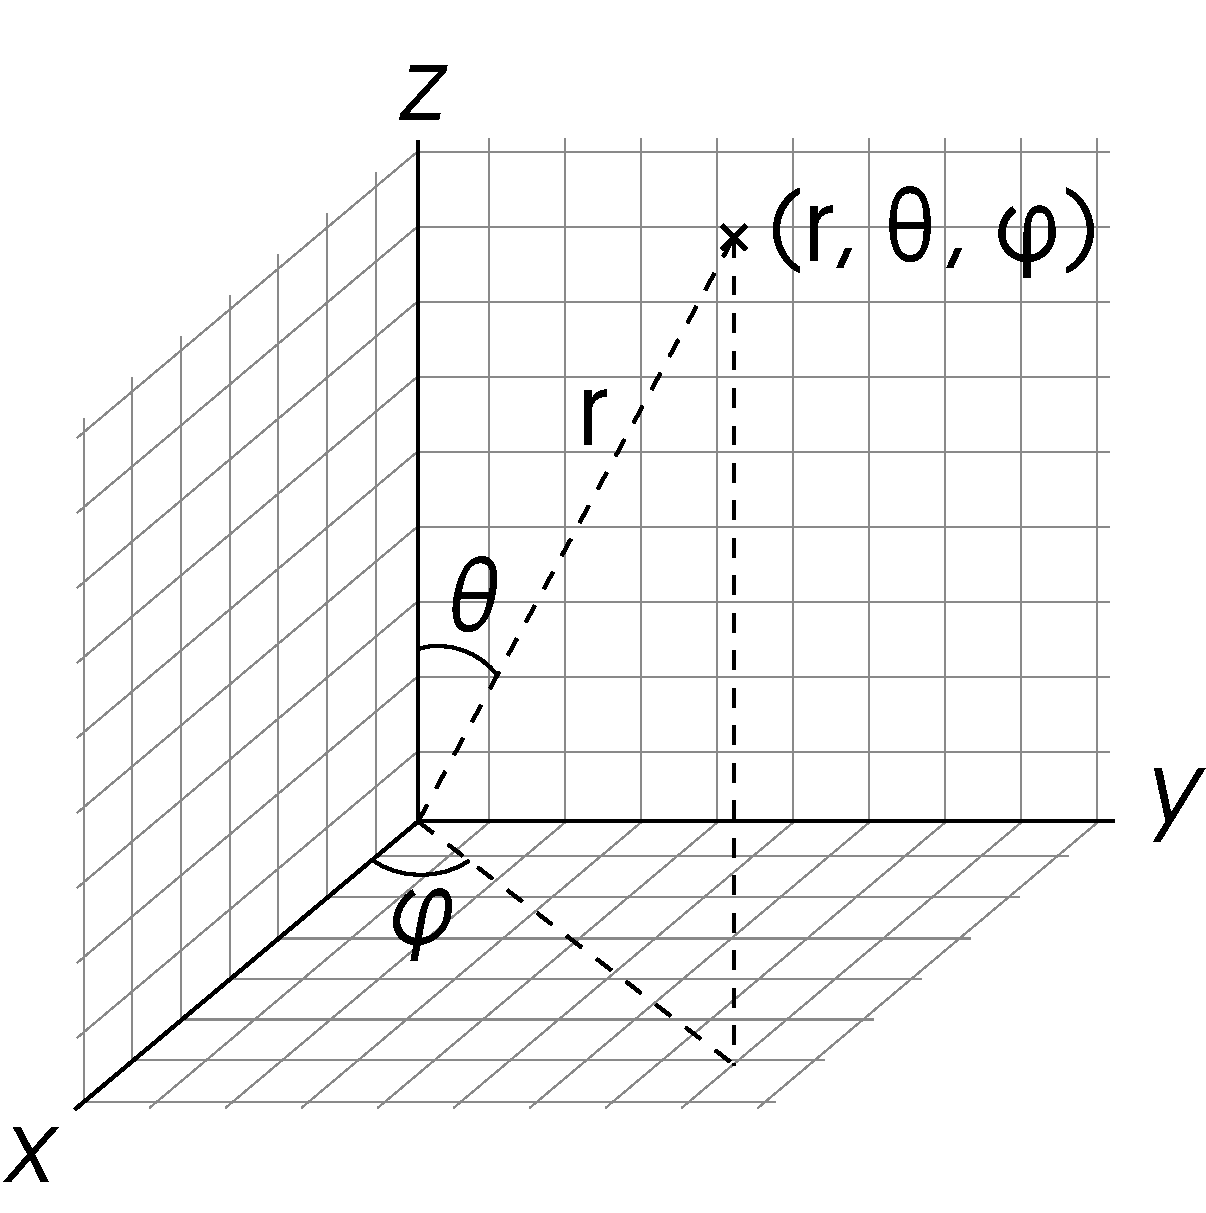
\includegraphics[width=0.50\linewidth]{fig/3D_Spherical}
    \caption{Spherical coordinates \((r, \theta, \phi)\). Radial distance \(r\), polar angle \(\theta\) (theta), and azimuthal angle \(\phi\) (phi). Source: \cite{WikiSpherical}.}
    \label{fig:3D_Spherical}
\end{figure}

And the coordinate transform equations to and from the cartesian coordinate system are:

\begin{align}
    x &= r \sin{\theta}\cos{\phi}, \label{eq:x(r,theta,phi)} \\
    y &= r \sin{\theta}\sin{\phi}, \label{eq:y(r,theta,phi)}\\
    z &= r \cos{\theta}, \label{eq:z(r,theta,phi)}
\end{align}

and

\begin{align}
    r &= \sqrt{x^2 + y^2 + z^2}, \label{eq:r(x,y,z)}\\
    \theta &= \arccos{\frac{z}{r}}, \label{eq:theta(x,y,z)}\\
    % \arctan{\frac{y}{x}}, \qquad \theta  \in [0, 2\pi]
    \phi &= 
    \begin{cases}
    \arctan{\frac{y}{x}} & \text{if \(x \geq 0\) \qquad \qquad \ \ \ (Q1, Q4),}
    \\
    \arctan{\frac{y}{x}}+\pi & \text{if \(x \leq 0,\ y \geq 0\) \qquad (Q2),}
    \\
    \arctan{\frac{y}{x}}-\pi & \text{if \(x \leq 0,\ y \leq 0\) \qquad (Q3).}
    \end{cases} \label{eq:phi(x,y,z)}
\end{align}

where \(r \in [0, \infty]\), \(\theta \in [0, \pi]\) and \(\phi \in [0, 2\pi]\).

For the calculation of kinetic in the next section we will need the position vector, unit vectors in spherical coordinates, and the Jacobians.

The position vector in spherical coordinates is
\begin{align}
    \vec{r}(r, \theta, \phi) &= x \xhat + y \yhat + z \zhat \\
    \Leftrightarrow \vec{r}(r, \theta, \phi) &= r \sin{\theta}\cos{\phi} \xhat + r \sin{\theta}\sin{\phi} \yhat + r \cos{\theta} \zhat. \label{eq:position-vec-spherical}
\end{align}

The various coordinate derivatives of the position vector is
\begin{align}
    \pd{\vec{r}}{r} &= \sin{\theta}\cos{\phi} \xhat + \sin{\theta}\sin{\phi} \yhat + \cos{\theta} \zhat \quad &\text{and} \quad &\left| \pd{\vec{r}}{r} \right| = 1 \label{eq:position-derived-r} \\
    \pd{\vec{r}}{\theta} &= r \cos{\theta}\cos{\phi} \xhat + r \cos{\theta}\sin{\phi} \yhat - r \sin{\theta} \zhat \quad &\text{and} \quad &\left| \pd{\vec{r}}{\theta} \right| = r \label{eq:position-derived-theta} \\
    \pd{\vec{r}}{\phi} &= -r\sin{\theta}\sin{\phi} \xhat + r\sin{\theta}\cos{\phi} \zhat \quad &\text{and} \quad &\left| \pd{\vec{r}}{\phi} \right| = r\sin{\theta} \label{eq:position-derived-phi}
\end{align}

So the unit vectors in spherical coordinates are
\begin{align}
    \rhat = \dfrac{\pd{\vec{r}}{r}}{\left| \pd{\vec{r}}{r} \right| } &= \sin{\theta}\cos{\phi} \xhat + \sin{\theta}\sin{\phi} \yhat + \cos{\theta} \zhat \label{eq:r-hat}\\
    \thetahat = \dfrac{\pd{\vec{r}}{\theta}}{\left| \pd{\vec{r}}{\theta} \right| } &= \cos{\theta}\cos{\phi} \xhat + \cos{\theta}\sin{\phi} \yhat - \sin{\theta} \zhat \label{eq:theta-hat}\\
    \phihat = \dfrac{\pd{\vec{r}}{\phi}}{\left| \pd{\vec{r}}{\phi} \right| } &= -\sin{\phi} \xhat + \cos{\phi} \zhat \label{eq:phi-hat}
\end{align}

\subsection{HR4B Equations of Motion}
We will follow the 5-step process of arriving at Hamilton's equations outlined in \cref{apx:hamiltons}.

\subsubsection{Step 1: Lagrangian \(L\)}
The kinetic energy of the system is
\begin{align}
    T = \frac{1}{2} m_s v^2.
\end{align}

In general the total derivative of a vector is:

\begin{align}
    \vec{v} &= \od{\vec{r}}{t} = \sum\limits_{i} \pd{\vec{r}}{q_i} \od{q_i}{t}, \\
      &= \sum\limits_{i} \left|\pd{\vec{r}}{q_i}\right| \frac{\pd{\vec{r}}{q_i}}{\left|\pd{\vec{r}}{q_i}\right|} \od{q_i}{t}, \\
      &= \sum\limits_{i} \left|\pd{\vec{r}}{q_i}\right| \od{q_i}{t} \unitvector{q}_i, \\
      &= \sum\limits_{i} \left|\pd{\vec{r}}{q_i}\right| \dot{q_i} \unitvector{q}_i,
    \end{align}

where we have used that a unit vector for any coordinate system is \(\frac{\pd{\vec{r}}{q_i}}{\left|\pd{\vec{r}}{q_i}\right|} = \unitvector{q}_i\).
We can now use the derivatives of the position vector we found earlier in \cref{eq:position-derived-r,eq:position-derived-theta,eq:position-derived-phi}, to substitute for \(\left|\pd{\vec{r}}{q_i}\right|\). We don't have to substitute in \(\unitvector{q}_i\) since our unit vectors are orthogonal, so they will yield either 0 or 1 when we square \(v\). So for the spherical coordinates we get:

\begin{align}
    \vec{v} = \dot{r}\rhat + r\dot{\theta}\thetahat + r\sin{\theta}\,\dot{\phi}\phihat
\end{align}

so

\begin{align}
    v^2 = \dot{r}^2 + r^2\dot{\theta}^2 + r^2\sin^2{\theta}\,\dot{\phi}^2
\end{align}

so we get

\begin{align}
    T = \frac{1}{2} m_s (\dot{r}^2 + r^2\dot{\theta}^2 + r^2\sin^2{\theta}\,\dot{\phi}^2).
\end{align}

The gravitational potential is \todoref{find some non-wikipedia reference here}

\begin{align}
    V = -G m_s \sum\limits_{i} \frac{M_i}{\left| \vec{r} - \vec{r_i} \right|}
\end{align}

So we finally get the Lagrangian

\begin{align}
    L &= T - V \\
    \Leftrightarrow L &= \frac{1}{2} m_s (\dot{r}^2 + r^2\dot{\theta}^2 + r^2\sin^2{\theta}\,\dot{\phi}^2) + G m_s \sum\limits_{i} \frac{M_i}{\left| \vec{r} - \vec{r_i} \right|}
\end{align}

\subsubsection{Step 2: Generalized Momenta \(p_i\)}


\subsection{Equations of Motion}


\subsection{Numerical Algorithm}
